%% This is an example first chapter.  You should put chapter/appendix that you
%% write into a separate file, and add a line \include{yourfilename} to
%% main.tex, where `yourfilename.tex' is the name of the chapter/appendix file.
%% You can process specific files by typing their names in at the 
%% \files=
%% prompt when you run the file main.tex through LaTeX.
\chapter{Introduction}\label{intro-ch}

\section{Spark and MapReduce}


New data processing systems such as Spark and MapReduce have been designed to help process the increasing amount of data. 
Instead of relying on just one powerful computer, these systems use many computers due to lower costs and increased scalability and fault tolerance. 
Because these systems are distributed in nature, they have stages (shuffle stages) where they transfer information between jobs. 
.
\section{Shuffle} 

We will use MapReduce to explain the shuffle in more detail, but the main concepts still apply to Spark.

\subsection{Shuffle Introduction}
In the first stage of MapReduce, the map phase, the data is loaded onto different computers and computation is performed on it that results 
in a group of key value pairs. The final phase of MapReduce,the reduce phase, assumes that all key-value pairs with the same
key are grouped together onto the same machine. We call this property the shuffle guarentee. Thus, the shuffle phase, an intermediate phase that the system handles internally, transfers key value pairs to satisfy the shuffle guarentee. 
\\

Figure~\ref{fig:shuffle_basic} display the inner workings 
of the shuffle phase in MapReduce. For instance, a programmer may  want to count the 
number of letters in a distributed file. The mappers will each load part of the distributed file and count the number of
letters in it. However, we need to aggregate this and 
thus all the counts for letter a will be sent to worker1, letter b will be sent to worker 2,
letter c will be sent to worker c. These reducers will then promptly aggregate the counts that they receive from the 
mappers.

\begin{figure}[h]
\begin{center}
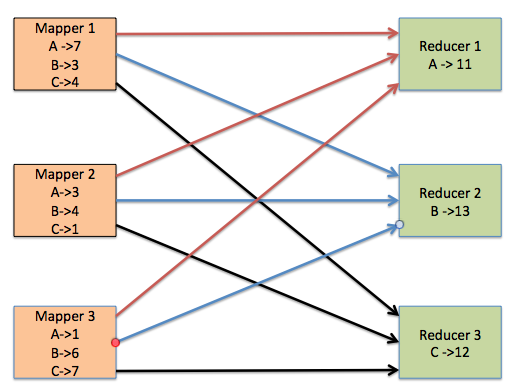
\includegraphics[scale=1.0]{./img/shuffle_basic.png}
\caption{Shuffle for Letter Count in Map Reduce}
\label{fig:shuffle_basic}
\end{center}
\end{figure}

Due of the huge amounts of keys, these systems do not transfer data on the granurality of keys.
Instead, they have the concept of partitions, which key value pairs with different keys. Programmers can pick different partitioning functions such as hash partitiong and range partitiong to map keys to partitions. Two keys that are identical are guarenteed to mapped to the same partition. As long as all the mappers partition their data in the same way and send each the corresponding partitions to the same reducer, the system satisfies 
the shuffle guarentee. 

\subsection {Shuffle Analysis}

Throughout the shuffle process, we want to balance the amount of data being sent to the reducers. 
These systems are constrained by the slowest worker, so generally we want to minimize the latencies of the slowest worker.
A more balanced workload for reducers reduces network latency for transferring the data and also reduces the execution time for the slowest worker.
Figure~\ref{fig:shuffle_unbalanced}, depicts a shuffle scenario that results in unbalanced paritions. Each mapper partition gets sent to the reducer id equal to the partition id mod the number of reducers. This protocol in theory should result in pretty balanced reducers but is not guarenteed to. As depicted, Reducer 3 receives 
40MB of data but Reducer 1 receives 90MB of data. However, if we knew the size of each partition after the mappers have run,
we could more intelligently balance the reducers. As seen in Figure~\ref{fig:shuffle_balanced}, with the same map output partitions, the system could attain complete balance
of 60MB for each reducer.


 \begin{figure}[h]
\begin{center}
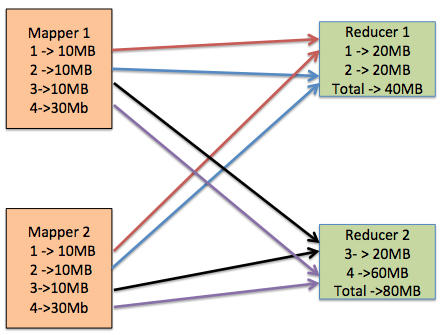
\includegraphics[scale=1.0]{./img/shuffle_unbalanced.png}
\caption{Unbalanced shuffle of partitions} 
\label{fig:shuffle_unbalanced.png}
\end{center}
\end{figure}

 \begin{figure}[h]
\begin{center}
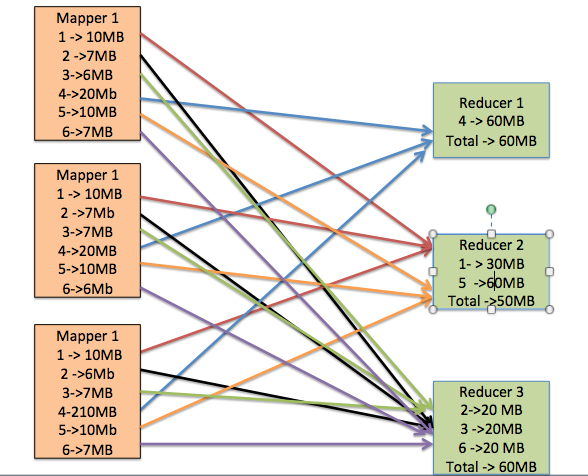
\includegraphics[scale=1.0]{./img/shuffle_balanced.png}
\caption{Balanced shuffle of partitions.}
\label{fig:shuffle_balanced.png}
\end{center}
\end{figure}

\section{Adaptive Scheduling of Joins}\label{intro-ch:eeg-overview}

\subsection{Join Basics}

A common operation in these data processing environments is a join.
A join basically combines two tables by finding intersections between
keys in respective columns. For instance, if we have   
Table\ref{table:join1} and Table\ref{table:join2} that we are trying to join based on the intersection
of key1 and key2, the resulting output is Table\ref{table:join3}   
\begin{table}[h!]
\centering
 \begin{tabular}{|c |c |c |c|}
  \hline
   Key1 & Value1 \\
  \hline
   a & 1 \\
  \hline
   a & 1 \\
  \hline
   b & 3 \\
  \hline
   c & 4 \\
  \hline
\end{tabular}
\caption{Table for Dataset 1}
\label{table:join1}
\end{table}

\begin{table}[h!]
\centering
 \begin{tabular}{|c |c|}
  \hline
   Key2 & Value2 \\
  \hline
   a & 5 \\
  \hline
   c & 7 \\
  \hline
\end{tabular}
\caption{Table for dataset 2}
\label{table:join2}
\end{table}

\begin{table}[h!]
\centering
 \begin{tabular}{|c |c |c|}
  \hline
   Key1 & Value1 & Value2  \\
  \hline
   a & 1 & 5 \\
  \hline
   a & 2 & 5 \\
  \hline
   c & 4 & 7 \\
  \hline
\end{tabular}
\caption{Table of Joined Data}
\label{table:join3}
\end{table}

\subsection{Shuffle Join}
The actual implementation of joins in MapReduce is very similar to the
shuffle scenario presented above. Instead of one dataset participating in the shuffle,
two datasets participate in the shuffle and ensure that their corresponding partitions 
are both sent to the same reducer.  
Figure \ref{fig:shuffle_join} details a shuffle join.
For both datasets, all of the keys that 
mapped to partition 1 were sent to the reducer 1 and this happens respectively for the rest of the partitions.

 \begin{figure}[h]
\begin{center}
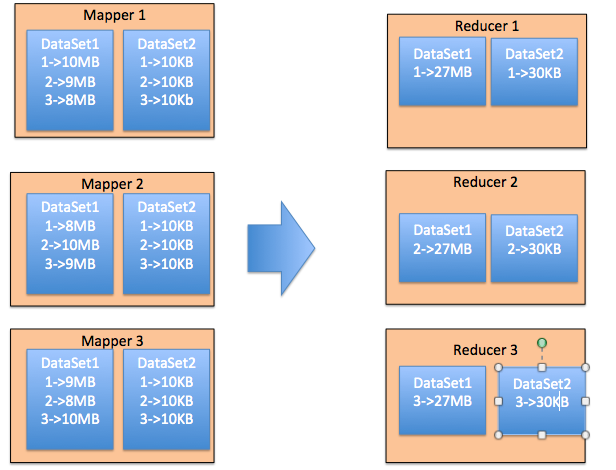
\includegraphics[scale=1.0]{./img/shuffle_join.png}
\caption{Typical Shuffle Join}
\label{fig:shuffle_join}
\end{center}
\end{figure}

\subsection {Broadcast Join}
The diagram above  may seem to imply that mappers and reducers
are different machines. However, this distinction is artificial and there are no seperate machines for mappers and reducers. 
Therefore, not all data in the shuffle stage is transferred over the network. In Figure~\ref{fig:shuffle_basic}, if Mapper 1
and Reducer 1 were the same machine, the key value pair A=7 would be read locally and not have to be the sent over the network.

In certain situations, it might make sense to keep all of dataset1 in place and transmit all of dataset 2 to each
machine in dataset 1. This method still provides correctness even though dataset 1 stays in place, because all partitions
of dataset 2 are sent. The advantages are that if dataset 2 is super small and dataset 1 can just stay in place, 
the network latency can be reduced. The following diagram \ref{fig:broadcast_join} demonstrates how data would be shuffled
using the broadcat join. Notice how the amount of data being transferred would be in the kiloybytes instead of the megabytes.

Broadcast Join is not always the optimal strategy. Because the entirety of dataset2 is sent to all partitions, the amount of computation
increases. Additionally, if the datasets are sufficiently the same size, than the amount of data transferred over the network will actually
increase because dataset 2 is sent in its entirety to every machine. 

Thus, when choosing join strategies it becomes clear that certain strategies are good in certain situations. Thus, it becomes imperative
to be able to pick the strategy after the mappers have run and we know the sizes of them.

 \begin{figure}[h]
\begin{center}
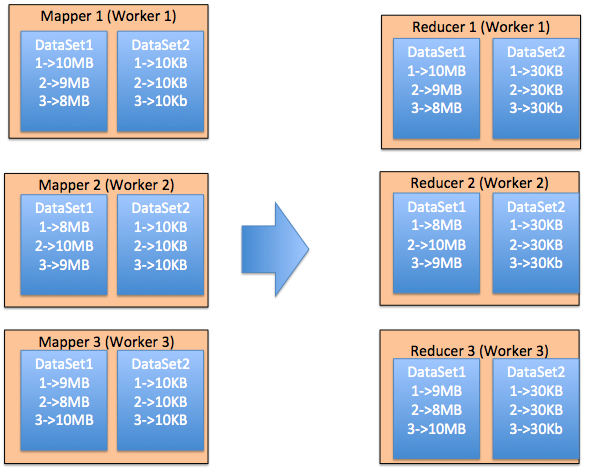
\includegraphics[scale=1.0]{./img/broadcast_join.png}
\caption{Broadcast Join}
\label{fig:broadcast_join}
\end{center}
\end{figure}


